\chapter{Introduction} \label{sec:intro}

In computer graphics, most images are typically stored as a sequence of dots in a rectangular grid (see Fig. \ref{fig:raster-images-upclose}). Each dot is called a pixel, a small part of an image that holds one specific colour, Photographs, also called natural images \cite{hoshyari2018perceptiondriven}, are one of, if not the most, common images that are stored in this manner. Many digital forms of art or any graphics work, such as paintings, posters, and icons, are also stored the same. Digital images stored in this manner are called \textit{raster images}. These images are stored in various image formats. The most commonly used formats are JPEG, GIF, BMP, TIFF, and PNG. Each have their pros and cons, from quality of the resulting image to the file size. Nevertheless, they all still accomplish the task of holding raster image data. Everything you see in the displays of devices such as laptops and mobile devices is a raster image. Computer displays are collections of pixels, in the common definition of a dot on the screen, which computers map images to to be able display them. This is the reason why \textbf{all} \textit{displayed} images are raster images.

\begin{figure}[h]
	\centering
	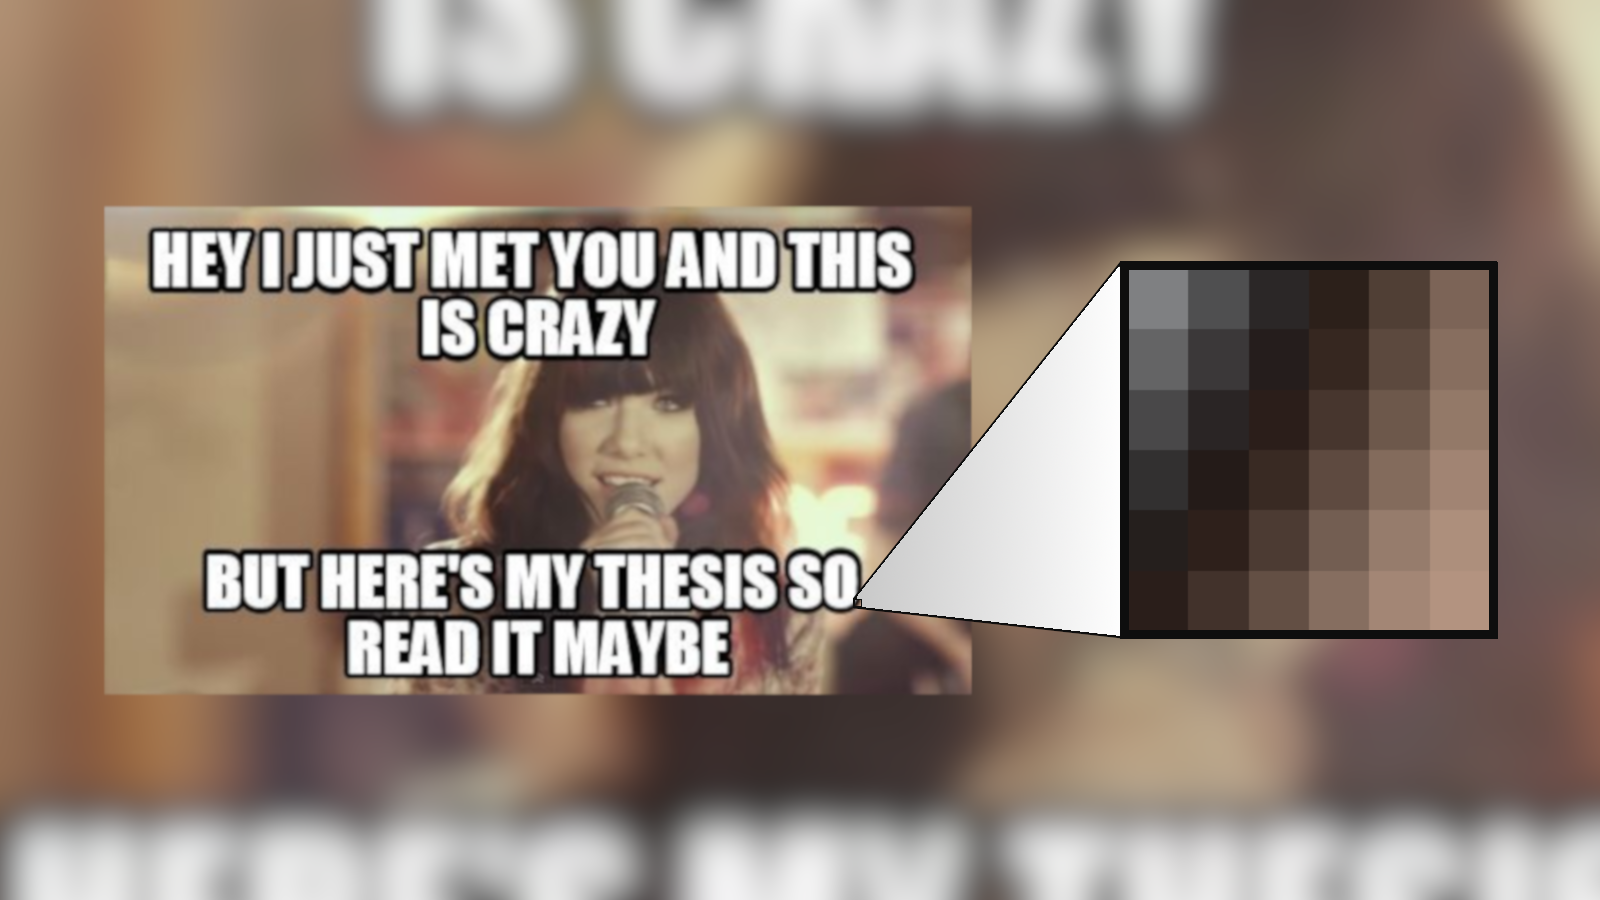
\includegraphics[scale=1.0]{images/chap01-introduction/raster-images-upclose.png}
	\caption{When zoomed in enough, each individual pixel of a raster image is visible. Meme image obtained from \protect\url{http://thesismemes.tumblr.com/post/73483120281}.}
	\label{fig:raster-images-upclose}
\end{figure}

A positive aspect of raster images is their simplicity. As mentioned earlier, raster images consists of a grid of pixels (also called a pixel matrix in other literature \cite{realtimevectorizationgpu}). This pixel grid can simply be assigned a combination of colour values to create an image. As such, working with raster images can be analogous to painting in the real world \cite{rastervsvector}. Given the right combinations of colours, we can produce natural images, i.e. photographs \cite{hoshyari2018perceptiondriven}. Intuitively, this means that we can store fine details in a raster image \cite{optimizedgradientmeshes}. This is in contrast to \textit{vector images}, which use a series of points and mathematical calculations to form lines and shapes. Vector images are unable to display lush colour depth and keep granularity, as found in raster images, as they use solid colours or gradients  \cite{rastervsvector}\cite{rastervsvectorgraphics}. There are studies that have been conducted in improving and utilizing \textit{gradient meshes}, a vector graphics primitive that allows for intricate colour gradients in regular quadrilateral meshes first introduced by Adobe Illustrator, to produce photorealistic vector images. However, as noted in the paper by Jian, S, Liang, L., Wen, F., and Shum, H., simple gradient meshes are insufficient to keep the fine details of images \cite{barendrecht2018locally}\cite{optimizedgradientmeshes}. It is also important to mention that vector graphics, despite represented as mathematical calculations, are still converted to raster format in a process called \textit{rasterization} for it to be displayed on-screen, since many modern screens are raster displays \cite{howdovectorgraphicswork}.

\section{The Problems of Raster Graphics}
With all the pros raster graphics have, it does not mean raster graphics are not without their caveats. Raster graphics have their own disadvantages which could affect the image quality and their use.

\begin{figure}[h]
	\centering
	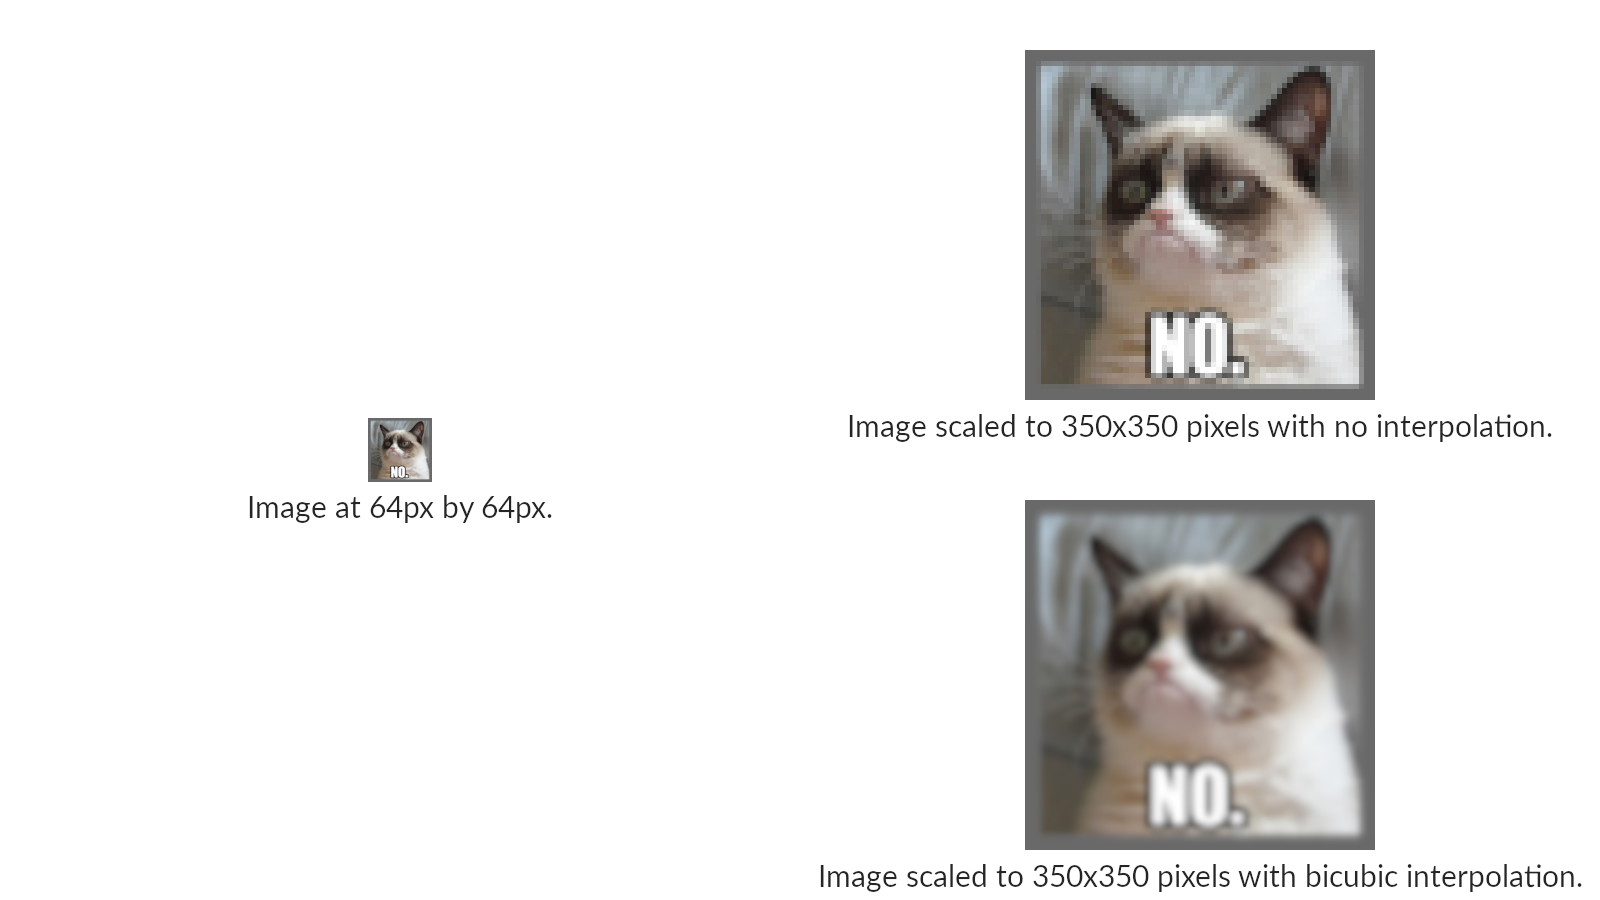
\includegraphics[scale=1.0]{images/chap01-introduction/raster-images-scaled.png}
	\caption{Different interpolation algorithms will produce different results. As seen in the image, the quality will also differ, from an image looking blocky to an image looking blurry. Cat meme image obtained from \protect\url{https://www.hercampus.com/school/uwindsor/school-thoughts-told-grumpy-cat-memes}.}
	\label{fig:raster-images-scaled}
\end{figure}

Raster graphics are \textbf{resolution-dependent}. This simply means that raster images are in their highest quality in the resolution they are initially created in and attempting to scale it up will gradually degrade the quality of the image as the image size or resolution grows larger. Rasters only have a finite number of pixels. Increasing the size of an image (also called upsampling \cite{hoshyari2018perceptiondriven} or single-image super resolution \cite{sisrbenchmark}) would entail moving the individual pixels into different locations depending on the scaling factor, the distance the individual pixels will be moved to horizontally and vertically. Upsampling will create empty pixels in between the shifted pixels when there is nothing done to substitute the empty pixels. This will create an unusable image \cite{resizingimages}. We can utilize interpolation to fill these empty pixels with colour. \textit{Classical} image upsampling approaches approximate colour and intensity values of these empty pixels are calculated based on the values of surrounding pixels, typically the shifted pixels. However, the specifics are dependent on the interpolation algorithm used in upscaling the images. Commonly used classical interpolation methods for resizing images include Nearest-Neighbour, Linear Interpolation, and Cubic Interpolation, which most, if not all, are readily available in popular raster image editing applications, such as Adobe Photoshop \cite{photoshopinterpolationmethods} and GIMP \cite{gimpinterpolationmethods}. The results produced by these interpolation algorithms typically suffer from blurring of sharp edges and ringing artifacts due to the fact that the algorithms do not assume anything about the data \cite{depixelizingpixelart}\cite{interpolationtechniquessurvey}. See Fig. \ref{fig:raster-images-scaled} for an example of blurring caused by scaling. There are adaptive image scaling techniques that consider image features such as edge information and texture to scale images with better quality than the classical methods. Examples of adaptive techniques are content-aware image resizing, seam curving, and warping-based methods. These techniques have their downsides as they take more computational time than their non-adaptive counterparts and may produce unexpected or even unsatisfactory results \cite{interpolationtechniquessurvey}. One of the latest advancements in upscaling images involves the use of artifical intelligence, specifically \textit{neural networks}, as found in the works of AI Gigapixel and by Yang, C. Ma, C. and Yang, M.. They produce high quality upscaled images and is a significant improvement over previous non-AI based upscaling techniques. However, they require high-end expensive hardware to produce results in the shortest amount of time possible. In the case of AI Gigapixel, a laptop with an integrated graphics card takes 20 minutes to produce a final high resolution image. For the work by Yang. C, Ma.C., and Yang. M., they utilized an Nvidia Titan Xp, a high-end GPU that costs \$1,200 as of November 18, 2018 \cite{titanxppage}, to upscale a 520x520px image 2x, 4x, and 8x its size, and took 0.8s, 2.1s, and 4.4s, respectively, to complete \cite{aigigapixelstory}\cite{progressivesisr}.

\section{Vectorization To The Rescue}
Vectorization is the process of converting raster images into vector images \cite{effectiveclipartimagevectorization}. Vector graphics uses collections of geometric primitives, such as points, curves, and points, and mathematical calculations to form an image \cite{rastervsvector}. Unlike raster graphics which uses a large pixel matrix (which will require large spaces without using proper image compression), vector graphics are able to smoothly scale to different resolutions, large or small, without any degradation in image quality \cite{realtimevectorizationgpu}\cite{barendrecht2018locally}. This makes them \textbf{resolution-independent}. Vector graphics innately have this property due to their reliance on mathematics, instead of context-free pixel grids. Each primitive have their own mathematic formulas which, obviously, stay the same no matter what the size of an image is. As such, the primitives can simply be re-rendered whenever the image is scaled \cite{rastervsvector}\cite{rastervsvectorgraphics}. Vector graphics also allow for easier editing \cite{hoshyari2018perceptiondriven}\cite{optimizedgradientmeshes}, as you only need to modify individual polygons, lines, and curves, instead of dealing with individual pixels like you normally would when using raster images editors.

\begin{figure}[h]
	\centering
	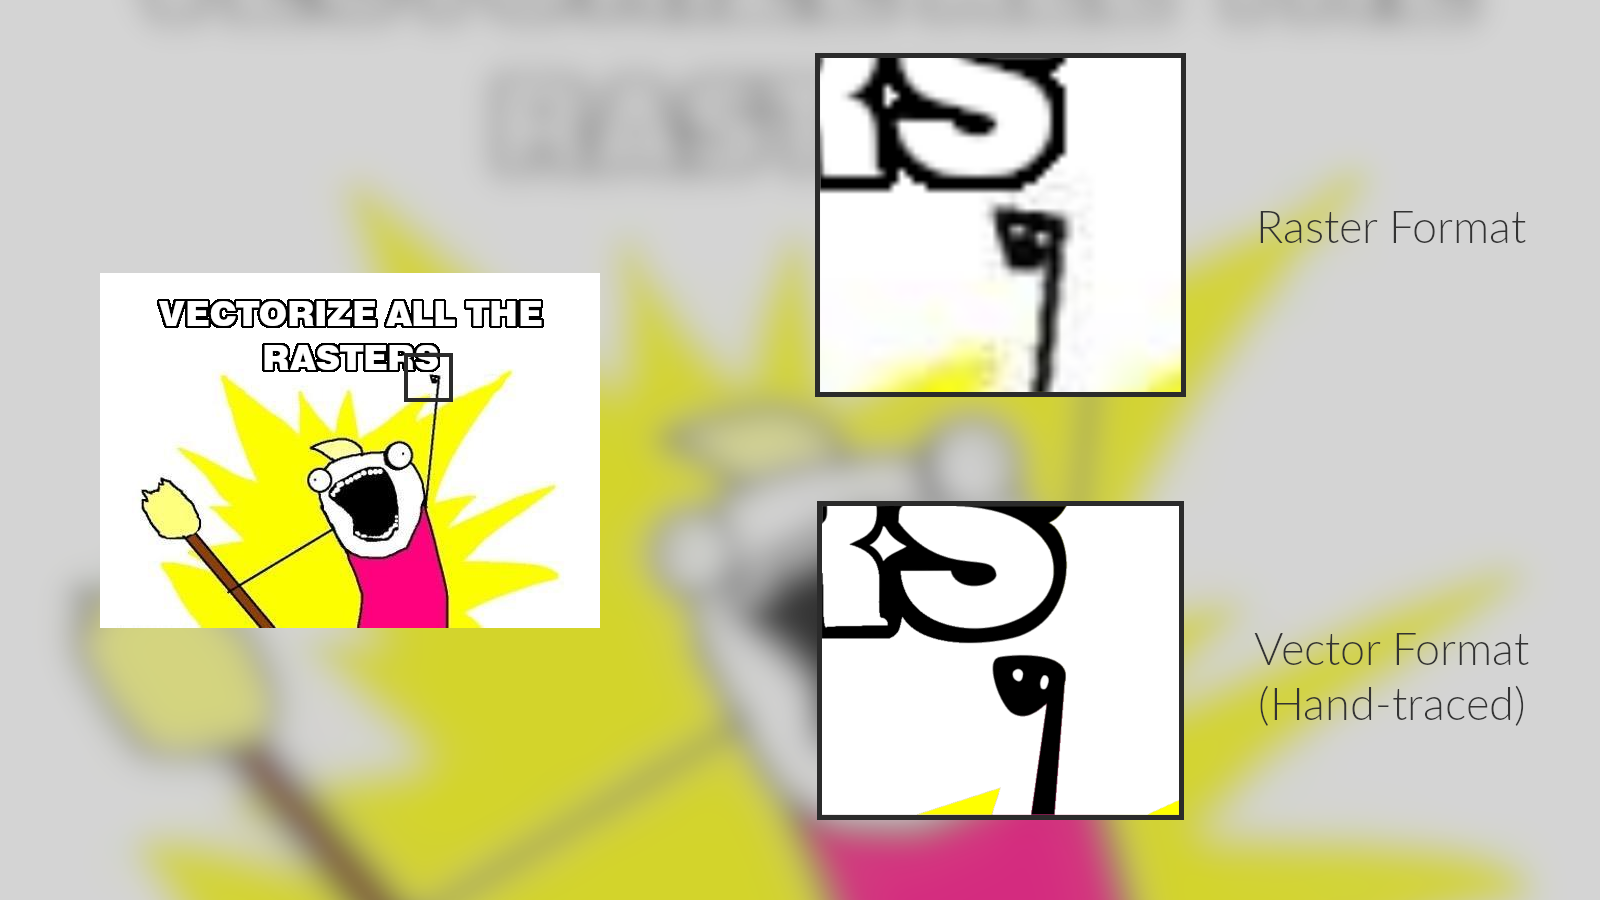
\includegraphics[scale=1.0]{images/chap01-introduction/raster-vs-vector.png}
	\caption{Zooming in closely at the same image, but one being in raster format (top right) and the other in vector (though hand-drawn; bottom left), quickly reveals the quality differences of both image formats. Raster images will show you individual pixels when close enough, but vectors will remain smooth.}.
	\label{fig:raster-vs-vector}
\end{figure}

Vectorization would often be done manually. In a study by Hoshyari, et. al. \cite{hoshyari2018perceptiondriven}, each of their raster images, which includes icons and small graphic illustrations, take 30-45 minutes to be vectorized by an artist. More than 7 million man hours are being spent on vectorizing raster graphics in the United States every year, according to a survey in the PhD dissertation of J.R. Diebel entitled, "Bayesian image vectorization: The probabilistic inversion of vector image rasterization" \cite{effectiveclipartimagevectorization}. Demand is, therefore, there for a robust vectorization algorithm.

Vectorization have been applied in many cases including, but not limited to, 2D maps and natural images. There are multiple methods that can be utilized in the vectorization of raster images. Their results differ from one method to another and even from one input to another, as many vectorization methods are fine tuned to specific inputs, such as those by Hoshyari, S., et. al. (semi-structured images) \cite{hoshyari2018perceptiondriven}, Kopf, J. and Lischinski, D. (pixel art) \cite{depixelizingpixelart}, and Bessmeltsev, M. and Solomon, J. (line drawings) \cite{vectorizationoflinedrawingspolyvector}. Additionally, the ability to utilize GPUs for computational tasks has allowed parallelization of vectorization such as in the paper where a GPU was used to vectorize a video stream in real time \cite{realtimevectorizationgpu}.

Many vectorization methods target natural images. As noted by Hoshyari, S., et. al. many of these natural image vectorization methods utilize \textit{image segmentation} to identify the portions of the image that will be converted into geometric primitives. These primitives are then filled with solid colors (e.g. such as what was done by Birdal, T. and Bala, E. \cite{anovelmethodforvectorization}), gradient meshes (which are used in Adobe Illustrator and Corel CorelDraw \cite{optimizedgradientmeshes}\cite{barendrecht2018locally}), and/or diffusion curves (such was the case in the paper by Xie, G. Sun, X., Tong, X., and Nowrouzezahrat, D. \cite{hierarchicaldiffusioncurves}). These vectorization methods produce differing results whose image qualities vary. Some results are as close as possible to the original raster image. Typically, gradient meshes and diffusion curves were utilized to achieve these results \cite{hierarchicaldiffusioncurves}\cite{optimizedgradientmeshes}\cite{barendrecht2018locally}. Others produce results with obvious colour segmentations, as seen in results that purely utilize solid colours (see \cite{anovelmethodforvectorization} for an example).

Natural images are not the only raster images that are being vectorized. Images called semi-structured images are also candidates for image vectorization. \textit{Semi-structured images} (SSIs) are images that consists of distinctly coloured regions and have well-defined boundaries \cite{hoshyari2018perceptiondriven}. Logos, cartoons, clip art, computer icons, and even simple graphical illustrations (such as flat 2D art) can considered to be semi-structured images. 60\% of the 10 million images to be vectorized are semi-structured images \cite{effectiveclipartimagevectorization}. This makes the demand for vectorizing these types of images evident. Various methods for vectorizing semi-structured images have been proposed by numerous papers. The common methodology of these proposals is that they attempt to fit curves or Bezier splines on the boundaries of each region in SSIs and fill in the appropriate colour. However, each of these methods naturally have their own unique ways of fitting curves. In the work of Kopf, J., and Lischinski, D. \cite{depixelizingpixelart}, they use similarity graphs and additional intermediate steps in identifying the regions of an image, though their work is targeted at pixel art. Another paper by Yang, M., et. al. would directly optimize the shapes of individual Bezier segments connecting each boundary transition vertices to produce high fidelity vectorized images \cite{hoshyari2018perceptiondriven}\cite{effectiveclipartimagevectorization}. The work by Hoshyari, S., et. al. can be seen as a complement to the aforementioned paper. Their work utilizes human perceptual cues, primarily guided by Gestalt psychology, to produce vectorizations of semi-structured images that align much more closely to what viewers expect from a raster image \cite{hoshyari2018perceptiondriven}.

An alternative method we can perform for image vectorization is to use machine learning via convolutional neural networks, a type of neural network that is well suited for image classification for their ability to learn various image features \cite{useofcnnimageclassification}, to create vectorizations of semi-structured images by having the computer learn to produce Bezier curves of image region boundaries that align well with the expected vectorization. This is the method that this paper is proposing. A similar work, in that convolutional neural networks were for vectorization, to this is that of the paper of Simo-Serra, E., Iizuka, S., Sasaki, K., and Ishikawa, H. where they convert and simplify paper-and-pencil sketch drawings to vectorized images \cite{simplifyingsketchesviacnn}.

% Note: Maybe add here why raster images are simple in the context of image processing once we learn more about image processing.